\begin{frame}
\frametitle{Audience Poll: Challenges of Parallel Programming}
How many of you have written parallel programs that suffer from:
\begin{itemize}
\only<1>{\item Bad scaling?
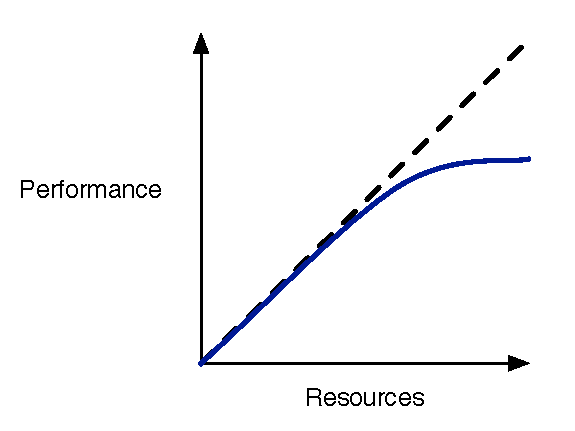
\includegraphics{../figures/bad_scalability.pdf}}
\pause
\only<2>{\item Sad scaling?
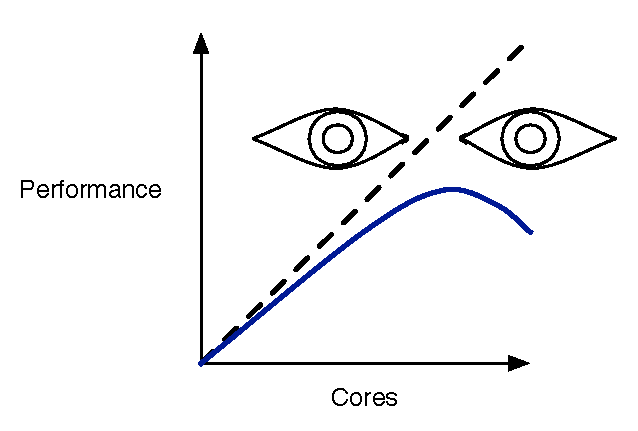
\includegraphics{../figures/sad_scalability.pdf}}
\pause
\item Bad scaling?
\item Races, deadlocks, etc: gremlins of shared state?
\pause
\item Limited to shared memory? GPU? No sharing allowed?
\pause
\item Design in terms of execution resources?
\pause
\item Independent tasks serialized or badly split across resources?
\pause
\item Application logic interwoven with parallelism optimizations?
\pause
\item Wasted energy?
\pause
\item Square peg logic in round hole framework abstractions?
\end{itemize}
\end{frame}
